\subsection{Critical Temperature}
    The evaluation of the Binder cumulant's intersections, yields the
    critical temperatures \(T_c\), which are plotted in
    fig. \ref{fig:Tc}\subref{sfig:Tc:RNG}\subref{sfig:Tc:GG}.
    Further in fig. \ref{fig:Tc}\subref{sfig:sumJ:RNG}\subref{sfig:sumJ:GG}
    the mean sum of the coupling constants to all neighbors \(\avg{\sum_{\avg{i,j}} J_{ij}}\)
    is plotted which is evidently correlated with \(T_c\).
    That is plausible, because \(T_c\) is dependend on the coupling
    constant \(J\) (compare \eqref{eq:exactTc}).\\
    It seems reasonable to normalize the values of \(T_{c}\) by
    \(\avg{\sum_{\avg{i,j}} J_{ij}}\) which yields the diagramms fig.
    \ref{fig:Tc}\subref{sfig:Tc_norm:RNG}\subref{sfig:Tc_norm:GG}.
    \begin{figure}[htbp]
        \centering
        \subfigure[][]
        {
            \label{sfig:Tc:RNG}
            \includegraphics[width=0.45\textwidth]{plots/RNG_Tc}
        }
        \subfigure[][]
        {
            \label{sfig:Tc:GG}
            \includegraphics[width=0.45\textwidth]{plots/GG_Tc}
        }

        \subfigure[][]
        {
            \label{sfig:sumJ:RNG}
            \includegraphics[width=0.45\textwidth]{plots/RNG_sumJ}
        }
        \subfigure[][]
        {
            \label{sfig:sumJ:GG}
            \includegraphics[width=0.45\textwidth]{plots/GG_sumJ}
        }

        \subfigure[][]
        {
            \label{sfig:Tc_norm:RNG}
            \includegraphics[width=0.45\textwidth]{plots/RNG_Tc_norm}
        }
        \subfigure[][]
        {
            \label{sfig:Tc_norm:GG}
            \includegraphics[width=0.45\textwidth]{plots/GG_Tc_norm}
        }
        \caption[Critical Temperature over different disturbance parameters]
        {
            Top: Critical temperatures over different
            disturbance parameters for
            \subref{sfig:Tc:RNG} the Relative Neighborhood Graph and
            \subref{sfig:Tc:GG} the Gabriel Graph.\\
            Middle: Mean sum of the coupling constants to all
            neighbors over different disturbance parameters for
            \subref{sfig:sumJ:RNG} the Relative Neighborhood Graph and
            \subref{sfig:sumJ:GG} the Gabriel Graph.\\
            Bottom: Normalized critical temperatures over different
            disturbance parameters for
            \subref{sfig:Tc_norm:RNG} the Relative Neighborhood Graph and
            \subref{sfig:Tc_norm:GG} the Gabriel Graph.
        }
        \label{fig:Tc}
    \end{figure}\\
    % I don't know what all that means...
    The Gabriel graph, which is shown on the right side of fig. \ref{fig:Tc},
    jumps from \(\sigma = 0\) to \(\sigma > 0\). This is easily explained
    by the definition of the Gabriel graph and it's aftereffects for
    the transition from \(\sigma = 0\). Visible in fig. \ref{fig:GG_sigma}
    a small change of sigma causes many new egdes to arise\footnote{See also \url{http://www.youtube.com/watch?v=PcVZ2pG11GI}}.
    To fully understand this, take four nodes forming a square. The edge
    across does not exist, because the other two nodes are on the edge
    of the lune. Move one node slightly into the square, causes the lune
    to get smaller, hence no other nodes are inside or on the edge of
    the lune anymore and the edge arises.
    \begin{figure}[htbp]
        \centering
        \subfigure[][]
        {
            \label{sfig:GG_sigma:zero}
            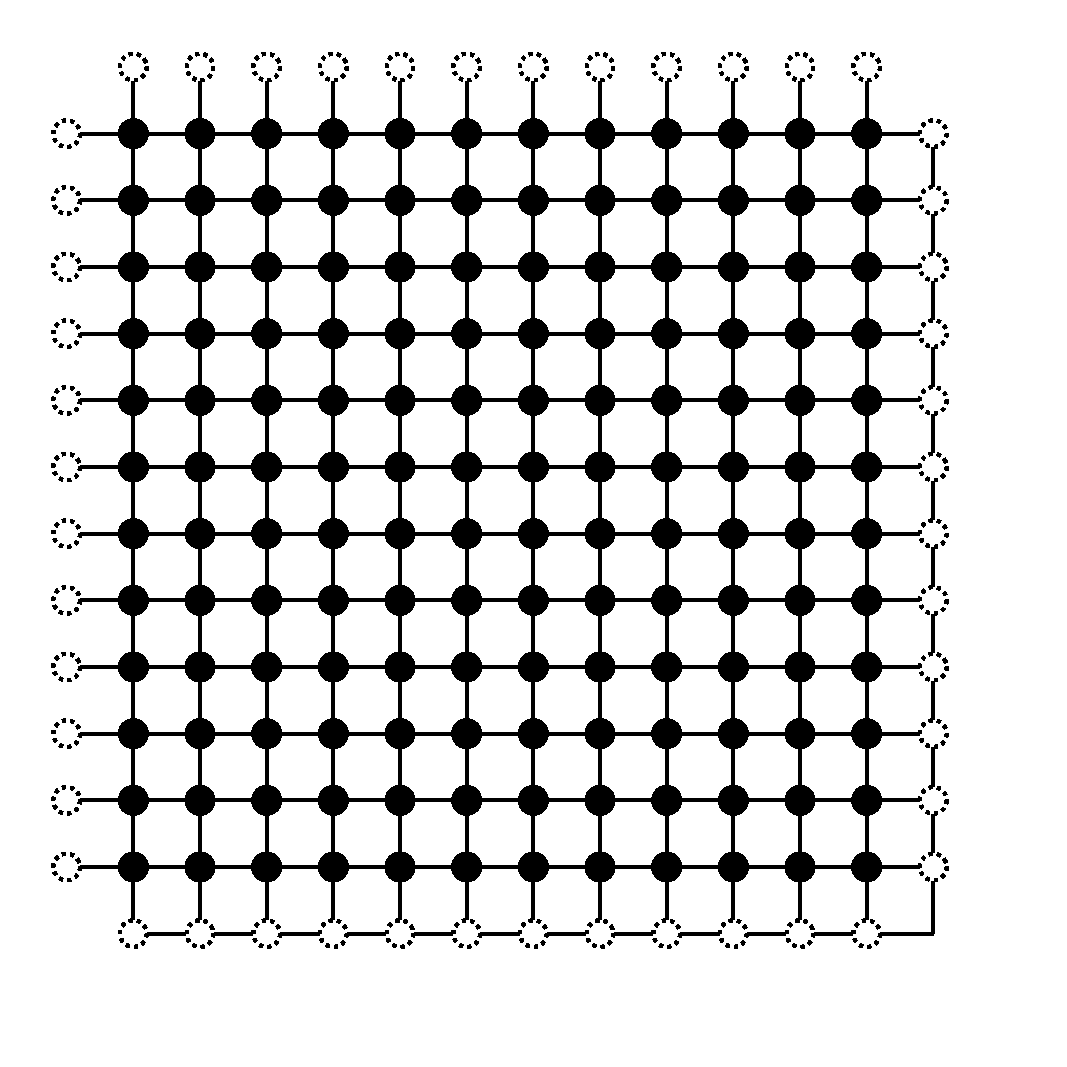
\includegraphics[width=0.45\textwidth]{images/GG/sigma_e0}
        }
        \subfigure[][]
        {
            \label{sfig:GG_sigma:notzero}
            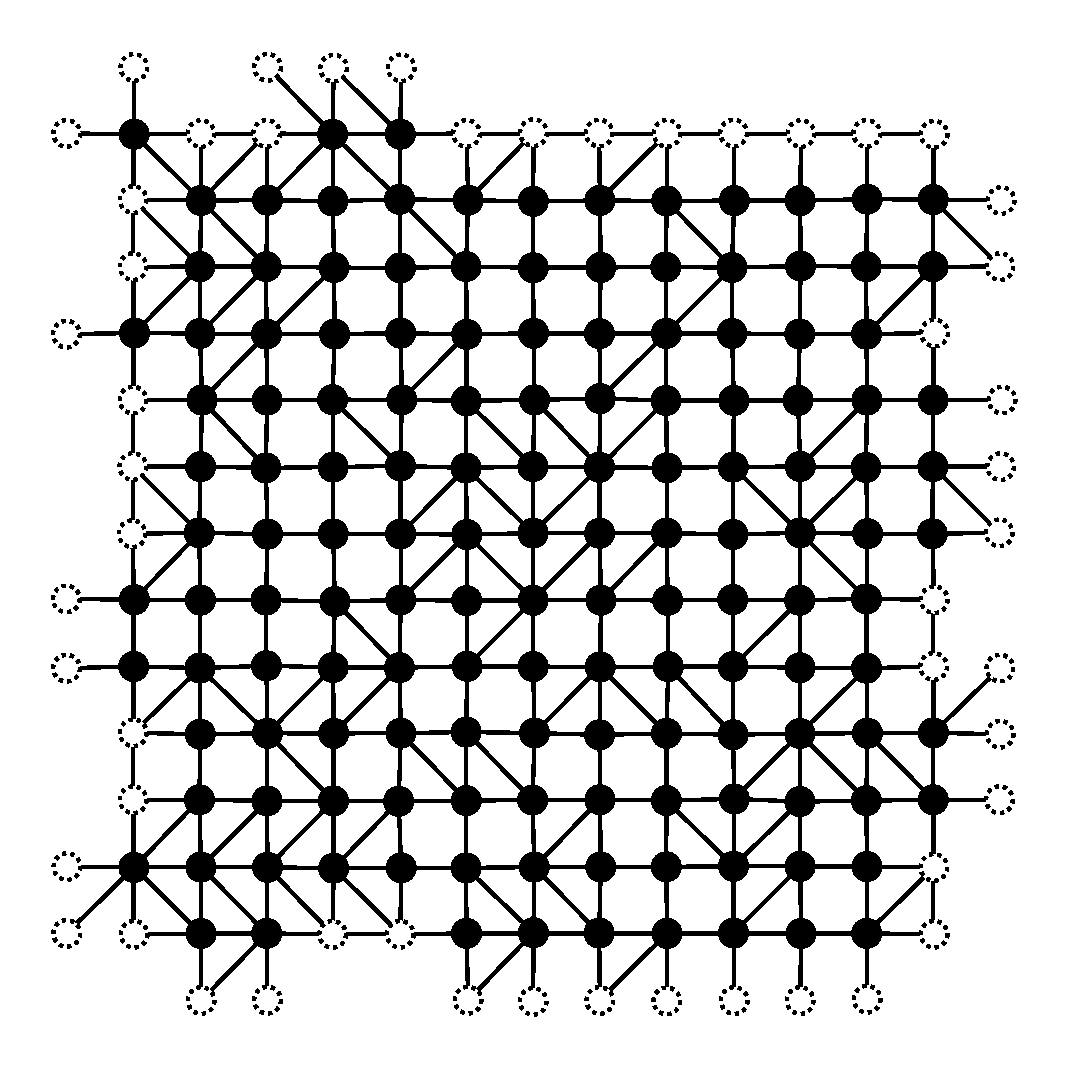
\includegraphics[width=0.45\textwidth]{images/GG/sigma_g0}
        }
        \caption[]
        {
            Gabriel graph with periodic boundary conditions for
                \subref{sfig:GG_sigma:zero} \(\sigma = 0\)
                \subref{sfig:GG_sigma:notzero} \(\sigma = 0.01\)
        }
        \label{fig:GG_sigma}
    \end{figure}\\
\subsection{Critical Exponents}
    For \(\sigma \in \{0,0.1,0.5\}\) a finite size scaling analysis was
    performed to determine the critical exponents \(\beta, \gamma, \nu\)
    using \texttt{autoscale.py} \cite{autoscale2009}. The values for
    \(\sigma = 0\) are analytically known \cite{Pelissetto2002}. The
    values for all other \(\sigma\) should be the same according to ???
    [citiation needed]. Like in tab. \ref{tab:critExp} to see, most values
    are matching the expectations. Most \(\beta\) seem to be a bit too
    big, but they are close enough to the expectations to be explained
    by the fact that small systems (\(L=32,64\)) were used for the
    analysis. [citation needed]
    \begin{table}[htbp]
        \center
        \begin{tabular}{l l l l l}
            \toprule
             & \multicolumn{1}{c}{\(\sigma\)} & \multicolumn{1}{c}{\(\nu\)} & \multicolumn{1}{c}{\(\gamma\)} & \multicolumn{1}{c}{\(\beta\)}\\
            \midrule
            exact (\cite[p. 59]{Pelissetto2002}) & \multicolumn{1}{c}{\(0\)} & \multicolumn{1}{c}{\(1\)} & \multicolumn{1}{c}{\(-\frac{7}{4}\)} & \multicolumn{1}{c}{\(\frac{1}{8}\)}\\
            \midrule
            Gabriel      & 0.0 & 1.008(4) & -1.735(2) & 0.1262(4)\\
                         & 0.1 & 1.02(1)  & -1.744(5) & 0.133(6) \\
                         & 0.5 & 1.009(8) & -1.75(1)  & 0.125(13)\\
            \midrule
            Relative N.  & 0.0 & 1.007(2) & -1.739(2) & 0.130(1) \\
                         & 0.1 & 0.99(1)  & -1.746(5) & 0.133(4) \\
                         & 0.5 & 1.00(2)  & -1.75(2)  & 0.143(13)\\
            \bottomrule
        \end{tabular}
        \caption{Critical exponents for different \(\sigma\)}
        \label{tab:critExp}
    \end{table}

    %~ <J>\(\sigma\), Anmerkung zur Anomalie des GG und der Ähnlichkeit von <J> zu \(T_c\)\\
%~
    %~ Erklärung zu Autokorreltationszeit \(\tau\) und Equilibrierungszeit \(t_eq\)\\
    %~ Darstellung von Suszeptibilität \(\chi\), spezifischer Wärme \(c\), mittlerer Magnetisierung \(<m>\) über Unordnungsparamter \(\sigma\)\\
    %~ Bestimmung der kritischen Punkte\\
        %~ Polyfit 4ten Grades durch Binder Kumulante \cite{Binder1981}\\
        %~ Finite Size Scaling Vergleich der Exponenten (AutoScale \cite{Melchert2009}, Vergleich \cite[S. 59]{Pelissetto2002})\\

